%\usepackage{subfig}

\chapter{Observational Procedures}

the full description of the survey is in: D. J. Sand et. al. 2011

MegaCam wide field imager on the CFHT (Canada-France-Hawii Telescope). The cluster sample consisted of 101 clusters within the range of redshifts from 0.05 < z< 0.55

58 clusters from the MENEACs (Multi-Epoch nearby cluster survey)

The meneacs clusters represent all clusters in the BAX X-ray cluster database that are observable for the CFHT

About 60 clusters, but we used only 30 for the final studies and paid special atention to 10, marked with *

G, U, I and R images


\begin{table}[]
\centering

\begin{tabular}{ccccc}
Cluster & $z$   & $\sigma(km/s)$ & $d(Mpc)$ & $\theta_{E}(")$ \\ \hline \hline
A1033   & 0.126 & 762            &  & 14.6155  \\
A1068*  & 0.138 & 740            &  & 13.5945  \\
A1132   & 0.136 & 727            &  & 13.1515   \\
A119*   & 0.044 & 875            &  & 21.0798   \\
A1413*  & 0.143 & 881            &  & 19.1569   \\
A1650   & 0.084 & 720            &  & 13.6758   \\
A1651   & 0.085 & 903            &  & 21.4876   \\
A1795   & 0.062 & 778            &  & 16.3514   \\
A2029*  & 0.077 & 1152           &  & 35.2776   \\
A2050   & 0.118 & 854            &  & 18.5258   \\
A2055   & 0.102 & 697            &  & 12.5642   \\
A2064   & 0.108 & 675            &  & 11.7048   \\
A2065*  & 0.073 & 1095           &  & 32.0110   \\
A2069   & 0.116 & 966            &  & 23.7574   \\
A2142*  & 0.091 & 1086           &  & 30.8756   \\
A2319*  & 0.056 & 1101           &  & 32.9563   \\
A2420   & 0.085 & ~800           &  & 16.8653   \\
A2440   & 0.091 & 766            &  & 15.3608   \\
A2597   & 0.085 & 682            &  & 12.2569   \\
A2627   & 0.126 & ~800           &  & 16.1096   \\
A2703   & 0.114 & ~800           &  & 16.3307   \\
A399    & 0.072 & ~800           &  & 17.1049   \\
A553    & 0.066 & ~800           &  & 17.2155   \\
A655*   & 0.127 & ~800           &  & 16.0911   \\
A754*   & 0.054 & ~800           &  & 17.4367   \\
A763    & 0.085 & ~800           &  & 16.8653   \\
A795    & 0.136 & ~800           &  & 15.9252   \\
A85*    & 0.055 & ~800           &  & 17.4182   \\
A961    & 0.124 & ~800           &  & 16.1464   \\
A990    & 0.144 & ~800           &  & 15.7778   
\end{tabular}
\caption{the redshifts of the clusters as given by C. Bildfell et. al. 2012 }
\label{my-label}
\end{table}

The original omages have dimesions of [11000:11000] pixels but since our relevant region is the center of the cluster where the BCG is located, we cut the images with dimension of [1000,1000] for the color analyisis and [4000:4000] to characterize the colors and discriminate between cluster and non-cluster members.

The INT images were multiple exposures so it was neccesary to make a mosaic of them using SWARP.

\section{Sextractor}

Segmentation image that will be used as a mask image (bad pixels) for galfit

We need to discriminate between field stars and the galaxies of the cluster so in order to do this, we used some of the parameters found by sextractor that allow us to constraint the fitted data. These are class-star, flux\_radius, and FWHM (full wicth half maximum). Class-star uses the neural network star/galaxy of sextractor that will give values close to 1 for stars and 0 for galaxies. flux\_radius, and FWHM are closely related to each other and give the radius which contains half of the light of the object so it will be small for stars and bigger for extended objects.



Color magnitude diagram for A1068

we used a zero point magnitude of 30

\begin{figure}[H]
\centering
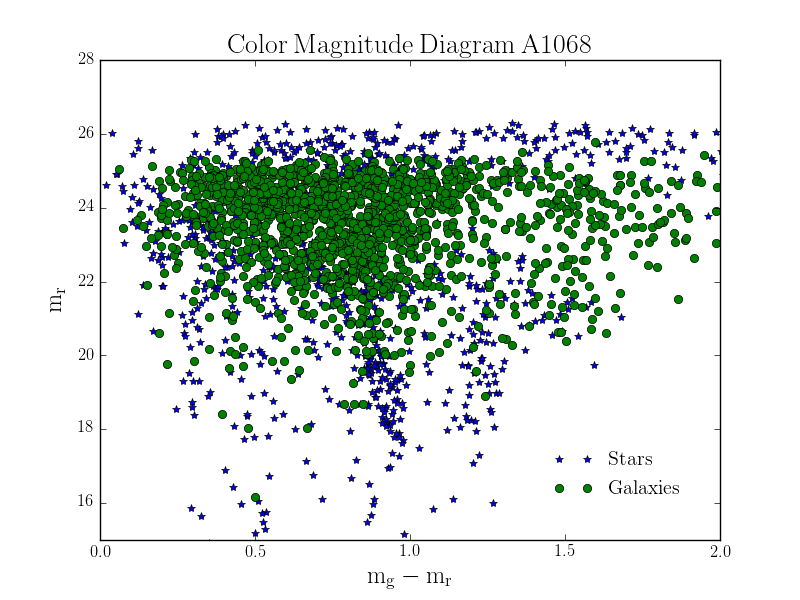
\includegraphics[width=12cm]{images/color mag.png}
\caption[M]{G}
\end{figure}

Mag vs flux rad to discriminate

\begin{figure}[H]
\centering
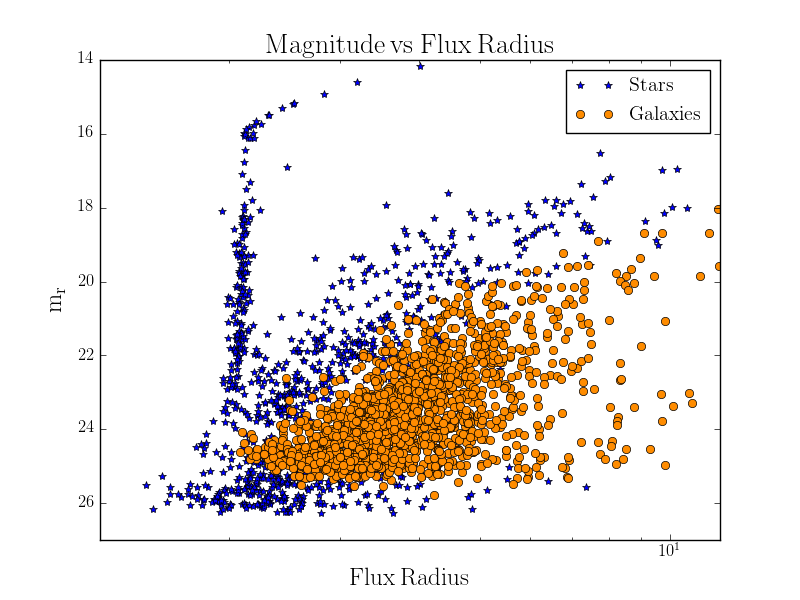
\includegraphics[width=12cm]{images/mag vs flux rad.png}
\caption[M]{G}
\end{figure}

\section{Galfit}

galfit fits two dimensional profiles so it is a useful tool to remove the light from the BCG and allow us to observe background objects

Fit sersic profiles with n=4 which is de vacouleurs profile. 

A first run gives us a rough idea of the true position of the center of the BCG so we can set this values in a second run for each cluster. We needed to combine different sersic parameters, as well as Fourier and bending modes for some of the BCGs.

We use the segmentation masks given by sextractor to mask bright objects in the fitting of the BCG

the fitting of many objects (not only the BCG)

the best results were given when we masked the innermost region of the BCG so the fitting will put more weight in the rest of the profile, thus reducing most of the light that hides the background objetcs.

we have to take into account the magnification bias

 The parameters C0, B1, B2, F1, F2, etc. listed below are hidden 
 from the user unless he/she explicitly requests them.  These can  be tagged on to the end of any previous components except, of 
 course, the PSF and the sky -- although galfit won't bar you from doing 
 so, and will just ignore them.  Note that a Fourier or Bending mode 
 amplitude of exactly 0 will cause GALFIT to crash because the 
 derivative image GALFIT computes internally will be entirely 0.  If a 
 Fourier or Bending amplitude is set to 0 initially GALFIT will reset it  
 to a value of 0.01.  To prevent GALFIT from doing so, one can set it to any 
 other value.

  Bending modes
B1)  0.07      1        Bending mode 1 (shear)
B2)  0.01      1        Bending mode 2 (banana shape)
B3)  0.03      1        Bending mode 3 (S-shape)

  Azimuthal fourier modes
F1)  0.07  30.1  1  1   Az. Fourier mode 1, amplitude and phase angle
F2)  0.01  10.5  1  1   Az. Fourier mode 2, amplitude and phase angle
F6)  0.03  10.5  1  1  Az. Fourier mode 6, amplitude and phase angle
F10)  0.08  20.5  1  1   Az. Fourier mode 10, amplitude and phase angle
F20)  0.01  23.5  1  1   Az. Fourier mode 20, amplitude and phase angle

  Traditional Diskyness/Boxyness parameter c
C0) 0.1         0       traditional diskyness(-)/boxyness(+)


\begin{figure}[H]
\centering
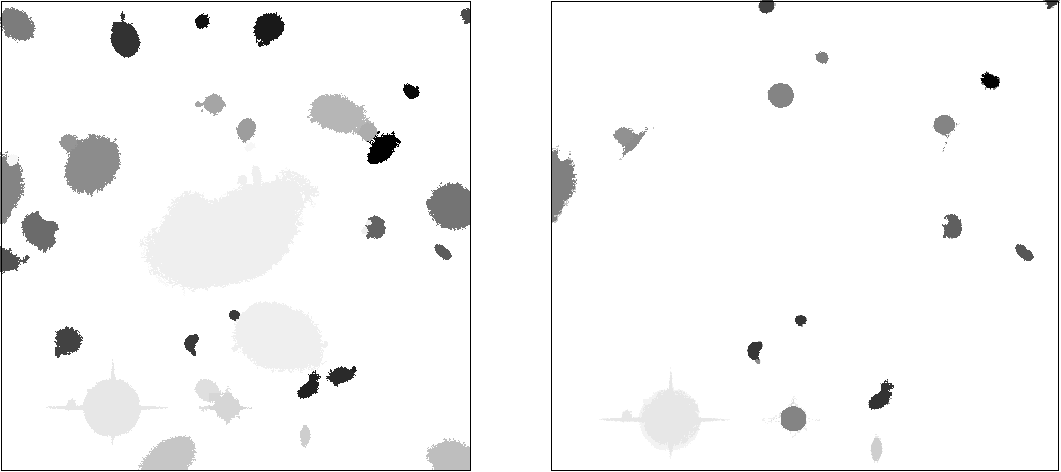
\includegraphics[width=12cm]{images/masks.png}
\caption[M]{G}
\end{figure}

\begin{figure}[H]
\centering
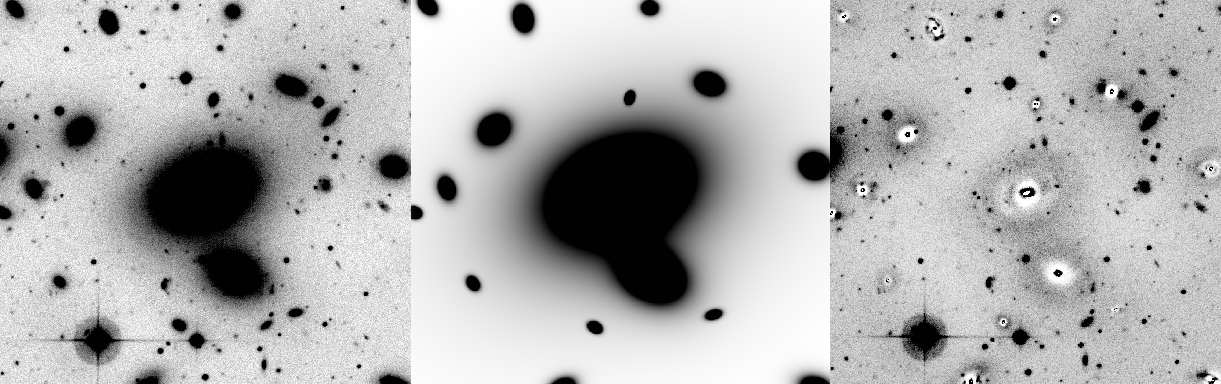
\includegraphics[width=15cm]{images/galfit.png}
\caption[M]{G}
\end{figure}

\section{Color images}


In er.  

Here we take an isothermal sphere to model the Einstein ring in a distance of background objects of z=1

\begin{figure}[H]
\centering
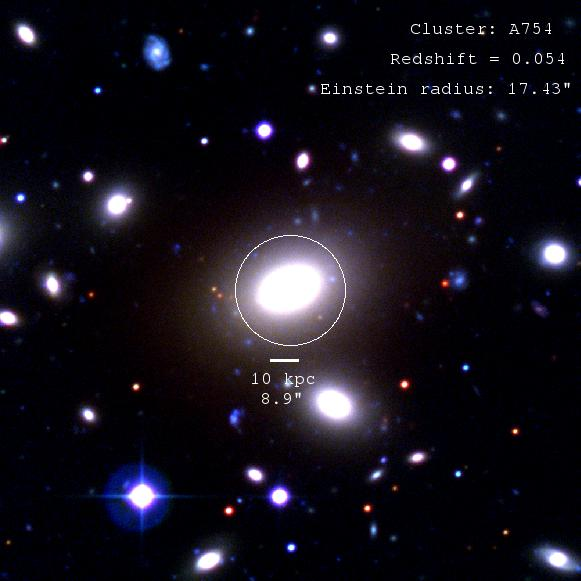
\includegraphics[width=12cm]{images/cA754.jpg}
\caption[M]{G}
\end{figure}

\begin{figure}[H]
\centering
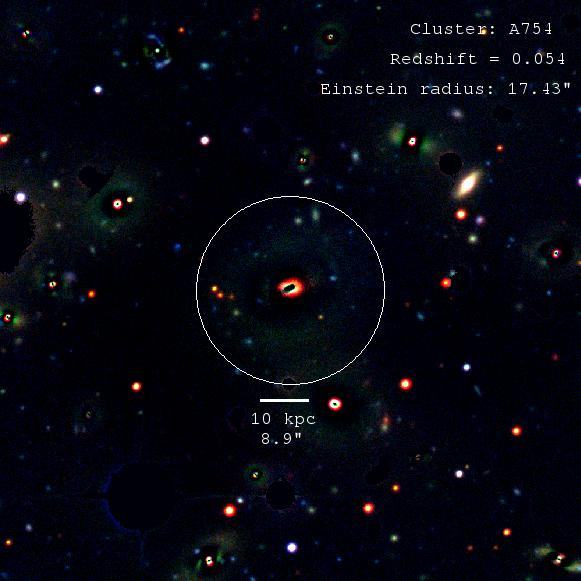
\includegraphics[width=12cm]{images/cA754_galfit.jpg}
\caption[M]{G}
\end{figure}


\section{Photometric Redshift}

(using as reference Benitez, Narciso 2000)